
	\newpage
% =========================================================	
	\section{Fixpunktiteration (LGS)}
% =========================================================
	
	\defi{
		\n 
		Beim letztem Mal haben wir Iterationsfunktionen kennengelernt und deren Nutzen im Bezug auf Fixpunkte erlernt.
		\n 
		Jetzt geht es darum, solch eine Iterationsfunktion für das Lösen von linearen Gleichungssystemen (=LGS) zu nutzen.
		Zu diesem Zwecke möchten wir ähnlich wie bei den Fixpunkten eine Iterationsvorschrift $\Phi(x)$ definieren, sodass wir iterativ die Lösung des Gleichungssystems annähern können.
	}

	\lbreak
% =========================================================
	\subsection{Vektoriteration}
% =========================================================
	
	\defi{
		\n 
		Wir probieren uns eine Iterationsfunktion herzuleiten. \\
		Die Idee ist, dass wir uns eine Matrix $M$ definieren, die möglichst gut $A$ approximiert, damit sie bei jedem Schritt die Lösung immer besser annähern kann.
	}
	
	\sbreak
	\methode{ Herleitung:
		\begin{align*}
			Ax &= b \\
			0 &= Ax - b \\
			0 &= M\inv(b - Ax) \\
			x &= x + M\inv(b - Ax)
		\end{align*}
		\begin{align} 
 			\Phi(x_k) = x_k + M\inv(b - Ax_k) = x_{k+1} 
 		\end{align}
	}

	\newpage
	\defi{
		\n 
		Für $M$ schauen wir uns folgende drei Vorschläge an. Wir haben im Hinterkopf, dass \\
			$M$ möglichst gut invertierbar sein muss, weil wir ja $M\inv$ brauchen
			und sie sollte die Matrix $A$ gut approximieren können (damit das Verfahren schnell konvergiert).
		\begin{itemize}
			\item Richardson: $M = \unitM$ \\
			Perfekt invertierbar aber approximiert die (beliebige) Matrix $A$ seeehr schlecht.
			\item Jacobi: $M = \diag(A)$\\
			Approximiert besser aber ist auch schlechter invertierbar.
			\item Gauß-Seidel: $M=A \cdot R$ \quad($R$ ist links untere Dreiecksmatrix) \\
			Approximiert die Matrix $A$ am besten und ist immer noch gut invertierbar.
		\end{itemize}
	}

	\sbreak
	\wichtig{
		\n 
		Eine volle Matrix zu invertieren kostet $\bigO(n^3)$. Das ist der Grund, warum wir als $M$ nicht einfach die Matrix $A$ nehmen, obwohl diese natürlich zur schnellsten Konvergenz führen würde. Irgendwie logisch, wir würden ja sonst das analytische ausrechnen und benötigten all das hier nicht.
	}

	\sbreak
	\defi{
		\n 
		Dadurch, dass wir beim ausrechnen immer $(b - Ax)$ benötigen, nennen wir dies ab sofort das \fat{Residuum} 
		\begin{align} 
 			r\st{k} = b - Ax\st{k} 
 		\end{align}
		Lasst euch von dieser Potenzschreibweise nicht ablenken. Dadurch, dass wir nachher mehrere Indizes brauchen, beschreibt hier die "Potenz" mit Klammern unseren Iterationsschritt und der "normale" Index unter der Zahl geschrieben beschreibt quasi die "Zeile" (also von oben nach unten um welchen Eintrag des Vektors / der Matrix es sich handelt).
		\n 
		Wir schreiben $a_{ii}$ für einen Diagonaleintrag der Matrix $A$, weil $ii$ die Position des Eintrages in der Matrix beschreibt ($i$ nach rechts und dann $i$ nach unten beschreibt für beliebiges $i$ die Diagonale der Matrix).
		\n 
		Wichtig ist, dass dies natürlich für jeglichen Größen $n\times n$ der Matrix funktioniert.
	}

	\newpage
	\subsubsection{Jacobi Verfahren}
	
	\methode{
		\n 
		Die $k$-te "Jacobi" Iteration:
		\begin{align} 
 			x\st{k+1} = x\st{k} &+ \diag(A)\inv\l(b - Ax\st{k}\r)
 		\end{align}
 		Wir teilen das auf in folgende Rechenschritte:
 		\begin{align}
 			r\st{k} &= b - Ax\st{k} \\
			y_i\st{k} &= \frac{1}{a_{ii}} \cdot r_i\st{k} \quad \quad \forall i \in [1, \dots, n]\\
 			x\st{k+1} &= y\st{k} + x\st{k} 
 		\end{align}
	}

	\sbreak
	\bsp{ \fat{Jacobi Verfahren}: $M = diag(A)$
		\n 
		Sei folgendes LGS gegeben:
		\begin{align*}
			\begin{bmatrix}
				1 & 3 \\
				2 & 2
			\end{bmatrix} \cdot 
			\nvector{
				x_0 \\ x_1
			} = 
			\nvector{
				2 \\ 2
			}
		\end{align*}
		1. Iteration von Jacobi mit dem Startvektor $x\st{0} = (0, 0)\trans$
		\begin{align*} 
 			r\st{0} &= b-Ax\st{0} = (2, 2)\trans - (0, 0)\trans = (2, 2)\trans \\
 			y_1\st{0} &= \frac{1}{a_{11}} \cdot r_1\st{0} = \frac{1}{1} \cdot 2 = 2 \\
			y_2\st{0} &= \frac{1}{a_{22}} \cdot r_2\st{0} = \frac{1}{2} \cdot 2 = 1 \\ \\
			x\st{1} &= x\st{0} + y\st{0} = 
			\nvector{
				0 \\ 0
			} 
			+ \nvector{
				2 \\ 1
			} 
			= \nvector{
				2 \\ 1
			}
		\end{align*}
		Jetzt käme die zweite Iteration, sprich man rechnet wieder alles von vorne nur jetzt mit dem neuen $x\st{1}$ anstelle vom alten $x\st{0}$
		\n 
		Und wenn man dies häufig genug macht, nähert sich das $x$ der Lösung unseres LGS an!
	}


	\newpage
	\subsubsection{Gauß-Seidel Verfahren}
	
	\defi{ Von Jacobi zu Gauß-Seidel:
		\n 
		Der Unterschied von Jacobi zum Gauß-Seidel Verfahren ist das sogenannte "in-place" Prinzip. Das bedeutet, dass wir im selben Iterationsschritt schon Informationen / Werte verwenden, die wir im selben Schritt erst ausgerechnet haben. Lustigerweise ist das dasselbe wie wenn wir einfach für $M$ die links untere Seite von $A$ nehmen würden (anstelle der Diagonalmatrix wie bei Jacobi).
		\n 
		Heißt, wenn wir den $i$-ten Eintrag von $r$ ausrechnen, verwenden wir für alle Einträge von $1$ bis $(i-1)$ nicht die Einträge vom alten Vektor, sondern direkt die neuen.
		\n 
		Wir trennen also $r = b - Ax\st{k}$ in zwei Teile auf.
		\begin{align} 
 			r_i\st{k} = b_i - \sum_{m = 1}^{i - 1}a_{im}x_m\st{k+1} - \sum_{m = i}^{n}a_{im}x_m\st{k} \quad \forall i = 1,\dots, n
 		\end{align}
		Diese Formel sieht viel komplizierter aus, als sie in der Praxis ist. Ich persönlich stelle es mir ähnlich eines Programmcodes vor, in dem neue Werte nicht separat abgespeichert werden, sondern direkt den jeweiligen Eintrag in unserer Lauf-variable $x$ überschreiben.
	}


	\sbreak
	\methode{
		\n 
		Die Methodik ändert sich also folgendermaßen:
		Die $k$-te "Gauß-Seidel" Iteration:
		\begin{align*} 
			\text{Für alle $i$ von $1$ bis $n$}: \\
			r_i\st{k} &= b_i - \sum_{m = 1}^{i - 1}a_{im}x_m\st{k+1} - \sum_{m = i}^{n}a_{im}x_m\st{k} \\
			y_i\st{k} &= \frac{1}{a_{ii}} \cdot r_i\st{k} \\
			x\st{k+1}_i &= y\st{k}_i + x\st{k}_i \\ \\
			\text{Zurück zur Schleife\dots}
		\end{align*}
	}

	\newpage
	\bsp{
		\n
		Selbes Beispiel wie bei dem Jacobi-Verfahren: 
		\begin{align*}
			\begin{bmatrix}
				1 & 3 \\
				2 & 2
			\end{bmatrix} \cdot 
			\nvector{
				x_0 \\ x_1
			} = 
			\nvector{
				2 \\ 2
			}
		\end{align*}
		1. Iteration von Gauß-Seidel mit dem Startvektor $x\st{0} = (0, 0)\trans$ \\
		Also (Programmcode--mäßig und damit informell):
		\begin{align*} 
			x_{\text{current}} := x_c &= x\st{0} = (0,0)\trans \\
			r\st{0}_1 &= b_1 - (Ax_c)_1 = 2 - 0 = 2 \\
			y_1\st{0} &= \frac{1}{a_{11}} \cdot r_1\st{0} = \frac{1}{1} \cdot 2 = 2 \\
			x\st{1}_1 &= (x_c)_1 + y\st{0}_1 = 0 + 2 = 2 \\ \\
			x_c &= (2, 0)\trans &\text{Alten Wert überschreiben} \\ \\
			r\st{0}_2 &= b_2 - (Ax_c)_2 = 2 - 4 = -2 \\
			y_2\st{0} &= \frac{1}{a_{22}} \cdot r_2\st{0} = \frac{1}{2} \cdot (-2) = -1 \\
			x\st{1}_2 &= (x_c)_2 + y\st{0}_2 = 0 - 1 = -1 \\ \\
			x\st{1} = x_c &= (2, -1)\trans &\text{Ein Schritt ist fertig}
		\end{align*}
		Hier käme jetzt also der nächste Schritt, der dann analog funktioniert.
	}

	\sbreak
	\defi{
		\n 
		Wir sehen am obigen Beispiel, dass Gauß-Seidel (für uns) deutlich schwieriger auszurechnen ist. Was man leider nicht sieht, aber dennoch der Fall ist: Gauß-Seidel nähert sich durch das "in-place" Prinzip der Lösung in aller Regel schneller an als Jacobi.
	}

	\newpage
% =========================================================	
	\subsection{Verfahren des steilsten Abstieges}
% =========================================================

	\defi{
		\n 
		Das sogenannte "Verfahren des steilsten Abstieges" (steepest descent) soll eine weitere Alternative sein, um iterativ ein LGS lösen zu können. Diese ist an den Fall angepasst, wenn $A$ symmetrisch und "positiv definit" (alle Eigenwerte $>0$) ist. \n
		Die grundlegende Idee ist es, dass wir uns die Funktion (offiziell Hyperfläche genannt) 
		\begin{align} 
 			f(x) = x\trans Ax - b\trans x + c 
 		\end{align}
 		definieren. Weil wenn wir das ableiten, erhalten wir 
 		\begin{align} 
 			\nabla f(x) = Ax - b 
 		\end{align} 
 		und die Nullstellen davon entsprechen dann $Ax = b$, unserem LGS. \\
	%}
		\begin{figure}[H]
			\centering
			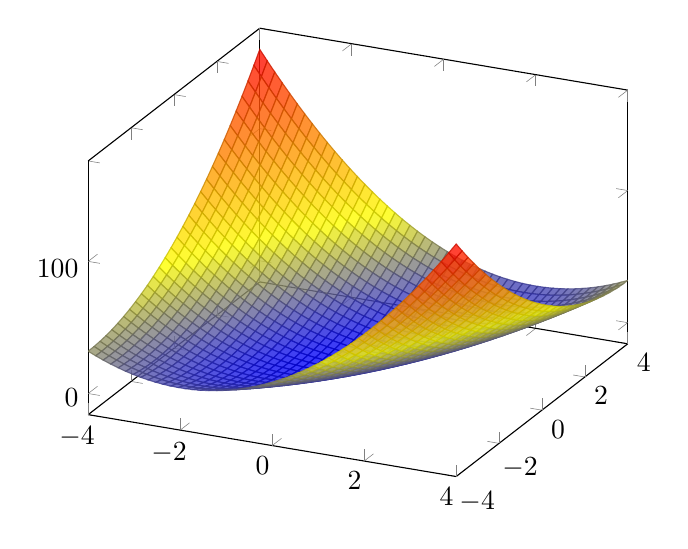
\begin{tikzpicture}
				\begin{axis}
					\addplot3[
					surf,
					opacity=0.8,
					samples=50, samples y=30,
					%samples=80, samples y=50,
					%colormap/whitered,
					%domain=-1:1,domain y=-2:6
					%domain=4:12,domain y=-20:-5
					domain=-4:4,domain y=-4:4
					%z buffer=sort,
					]
					%{x^2 - 4*x*y + y^2};
					%{2*x^2 - 1*x*y + 2*y^2 - x - 2*y};
					%{sin(0.5*x^2 - 0.25*y^2 + 3) * cos(2*x - exp(y) + 1)};
					%{4*x^2 + 5*x*y + 2*y^2 - 4*x + 12*y};
					{4*x^2 - 4*x*y + 2*y^2};
				\end{axis}
			\end{tikzpicture}
			\caption{Beispiel einer Hyperfläche.}
		\end{figure}
	}


	\newpage
	\methode{
		\n 
		In jeder Iteration dieses Verfahrens berechnet man folgende 3 Schritte:
		\begin{enumerate}
			\item Aktuelles Residuum: ("Schrittrichtung") 
			\begin{align} 
 				r\st{k} = b - Ax\st{k} 
 			\end{align}
			\item Optimale Schrittweite:
			\begin{align} 
 				\alpha\st{k} = \frac{r^{(k)\trans} \cdot r\st{k}}{r^{(k)\trans} \cdot A r\st{k}} 
 			\end{align}
			\item Aktuelles Zwischenergebnis:
			\begin{align} 
 				x\st{k+1} = x\st{k} + \alpha\st{k} \cdot r\st{k} 
 			\end{align}
		\end{enumerate}
	}

	\sbreak
	\bsp{
		\n 
		Sei folgendes LGS (aus obigem Beispiel) gegeben und der Startvektor $x\st{0} = (0, 0)\trans$
		\begin{align*}
			\begin{bmatrix}
				1 & 3 \\
				2 & 2
			\end{bmatrix} \cdot 
			\nvector{
				x_0 \\ x_1
			} = 
			\nvector{
				2 \\ 2
			}
		\end{align*}
		Wir berechnen die erste Iteration nach obiger Methode:
		\begin{align*}
			&r^{(0)} = b - Ax^{(0)} = 
			\nvector{
				2 \\ 2
			} \\
 			\alpha^{(0)} &= \frac{r^{(0)\trans} \cdot r^{(0)}}{r^{(0)\trans} \cdot A r^{(0)}} = \frac{8}{32} = \frac{1}{4} \\ 		
			x\st{1} = x\st{0} &+ \alpha\st{0} \cdot r\st{0} = (0, 0)\trans + \frac{1}{4} \cdot 
			\nvector{
				2 \\ 2
			} = \frac{1}{2} 
			\nvector{
				1 \\ 1
			}
		\end{align*}
		Hier käme die nächste Iteration und erfolgt völlig analog\dots
	}

	\newpage
	\defi{
		\n 
		Grafisch wird dieses Verfahren häufig so dargestellt, indem man die Höhenlinien der Hyperfläche als Kreise einzeichnet. Höhenlinien, weil ein Kreis bedeutet, dass alle Punkte auf dieser Kreislinie dieselbe Höhe (y-Wert) besitzen.
		\n 
		Das Verfahren konvergiert schneller, je gleichmäßiger es nach außen geht. Um genau zu sein braucht das Verfahren genau ein Schritt, falls die grafische Darstellung der Funktion (also die Höhenlinien) konzentrische Kreise bilden, also die Hyperfläche einem umgedrehten Kegel entspricht.
		\n 
		In der Praxis gleicht die grafische Darstellung meist eher weiten Ellipsen, weswegen dieses Verfahren genau so in der Praxis häufig recht langsam ist. Es gibt aber eine bessere Variante, das sogenannte "Conjugated gradient descent" (online nachschauen, wenn das Interesse geweckt hat).
	%}
	%
		\begin{figure}[H]
			\centering
				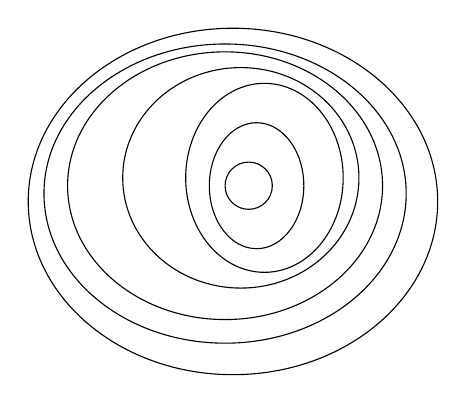
\begin{tikzpicture}
					\draw (0,0) ellipse (0.3cm and 0.3cm);
					\draw (0.1,0) ellipse (0.6cm and 0.8cm);
					\draw (0.2,0.1) ellipse (1.0cm and 1.2cm);
					\draw (-0.1,0.1) ellipse (1.5cm and 1.4cm);
					\draw (-0.3,0.0) ellipse (2.0cm and 1.7cm);
					\draw (-0.3,-0.1) ellipse (2.3cm and 1.9cm);
					\draw (-0.2,-0.2) ellipse (2.6cm and 2.2cm);
				\end{tikzpicture}
			\caption{Beispielhafte grafische Darstellung eines "steepest descent" Problems.}
		\end{figure}
		\noindent Die Schrittrichtung in einem Schritt ist dann einfach immer senkrecht zur momentanen Höhenlinie, da es der jeweils steilste Abstieg in dem Punkt ist.
%		Ein Bild hierzu wäre: \\
	}
	
%		Die Schrittrichtung ist immer senkrecht zur momentanen Höhenlinie.
%		%An diesem Bild sieht man auch schön grafisch, was bei den einzelnen Schritten passiert. Die Schrittrichtung entspricht immer senkrecht zur aktuellen "Höhenlinie", auch wenn diese natürlich nicht eingezeichnet ist. Gerade beim ersten Schritt, wo der Startpunkt genau auf einer Linie ist, kann man sehr gut erkennen, dass die Schrittrichtung orthogonal zu der Linie ist.
%		%\n 
%		%Und beim vierten Schritt (also von $x_3$ aus) erkennt man auch super, dass die Linie orthogonal zur Schrittrichtung ist.
%	}
